\section{Inputs \& outputs}
\subsection{}

\begin{frame}{Fixed-sized inputs (1/2)}
    \begin{columns}
        \begin{column}{0.816\textwidth}
            \begin{block}{}
                In some RNN applications, need to feed in constant \emph{fixed-size} $\z \in \Reals^l$
            \end{block}

            \begin{itemize}
                \item<+-> I.e., not a sequence
                \item $\z$ may be contextual information, or a latent vector
                \item Input sequence $\x_t$ might not even exist
                \item E.g., latent-to-sequence decoder
            \end{itemize}

            \begin{block}{Common approach 1}<+->
                Append \textcolor{Green4}{$\z$} to \emph{every} input $\x_t$
            \end{block}
        \end{column}
        \begin{column}{0.184\textwidth}
            \uncover<.->{\begin{tikzpicture}[node distance=7mm, auto]
    \node (state) [state] {$\s_t$};
    \node (input) [state, below=1cm of state, xshift=5mm] {$\x_t$};
    \node (latent) [latent, below=1cm of state, xshift=-5mm] {$\z$};
    \node (output) [state, above=of state] {$\y_t$};
    \node (loss) [function, above=of output] {$L$};
    \node (data) [data, above=of loss] {$\ETA_t$};
    \node (skip) [inner sep=0.5mm, above=1mm of state] {};
    \node (skip l) [coordinate, left=7mm of skip] {};
    \node (skip r) [coordinate, right=7mm of skip] {};
    \node (above) [coordinate, below=5mm of state] {};

    % Mux.
    \foreach \n in {input, latent} {
        \node (above \n) [coordinate, above=5mm of \n] {};
        \draw [path] (\n) -- (above \n);
    }

    \draw [ultra thick] (above input) -- (above latent);

    % Arrows.
    \draw [path] (above) -- node [label, pos=0.4, right] {$\f$} (state);
    \draw [path] (state) -- node [label, pos=0.6, right] {$\h$} (output);
    \draw [path] (output) -- (loss);
    \draw [path] (data) -- (loss);
    \draw [thick] (state) -| node [label, right, pos=0.7] {$\f$} (skip r) -- (skip);
    \draw [path] (skip) -- (skip l) |- (state);
\end{tikzpicture}
%%% Local Variables:
%%% mode: latex
%%% TeX-master: "../rnn"
%%% End:
}
        \end{column}
    \end{columns}
\end{frame}

\begin{frame}{Fixed-size inputs (2/2)}
    \begin{columns}
        \begin{column}{0.4\textwidth}
            \begin{block}{Common approach 2}
                Set initial state \textcolor{Green4}{$\s_0 = \z$}
            \end{block}
            \begin{block}{Common approach 3}
                Combine 1 \& 2
            \end{block}
            \begin{itemize}
                \item Downside: both force $\dim(\s_t) = \dim(\z)$
            \end{itemize}
        \end{column}
        \begin{column}{0.6\textwidth}
            \begin{tikzpicture}[node distance=7mm, auto]
    % States.
    \node (state0) [latent] {$\z$};
    \node (state1) [state, right=of state0] {$\s_1$};
    \node (state2) [state, right=of state1] {$\s_2$};
    \node (state3) [block, right=of state2] {$\cdots$};
    \node (state4) [state, right=of state3] {$\s_\tau$};

    % Inputs, outputs, losses.
    \foreach\i in {1, 2} {
        \node (input\i) [state, below=1 cm of state\i] {$\x_\i$};
        \node (output\i) [state, above=of state\i] {$\y_\i$};
        \node (loss\i) [function, above=of output\i] {$L$};
        \node (data\i) [data, above=of loss\i] {$\ETA_\i$};
    }

    \node (input3) [block, below=1cm of state3] {$\cdots$};
    \node (output3) [block, above=of state3] {$\cdots$};
    \node (loss3) [block, above=of output3] {$\cdots$};
    \node (data3) [block, above=of loss3] {$\cdots$};

    \node (input4) [state, below=1cm of state4] {$\x_\tau$};
    \node (output4) [state, above=of state4] {$\y_\tau$};
    \node (loss4) [function, above=of output4] {$L$};
    \node (data4) [data, above=of loss4] {$\ETA_\tau$};

    % Arrows.
    \foreach\i in {1, ..., 4} {
        \draw [path] (input\i) -- node [label, pos=0.4, right] {$\f$} (state\i);
        \draw [path] (state\i) -- node [label, pos=0.4, right] {$\h$} (output\i);
        \draw [path] (output\i) -- (loss\i);
        \draw [path] (data\i) -- (loss\i);
    }

    \foreach\i/\j in {0/1, 1/2, 2/3, 3/4} {
        \draw [path] (state\i) -- node [label, pos=0.4] {$\f$} (state\j);
    }
\end{tikzpicture}
%%% Local Variables:
%%% mode: latex
%%% TeX-master: "../rnn"
%%% End:

        \end{column}
    \end{columns}
\end{frame}

\begin{frame}{Fixed-size outputs}
    \begin{columns}
        \begin{column}{0.37\textwidth}
            \uncover<2->{\begin{tikzpicture}[node distance=7mm, auto]
    % States.
    \node (state2) [block] {$\cdots$};
    \node (state3) [state, right=of state2] {$\s_{\tau-1}$};
    \node (state4) [state, right=of state3] {$\s_\tau$};

    % Inputs.
    \node (input2) [block, below=of state2] {$\cdots$};

    \foreach\i/\j in {3/-1, 4/} {
        \node (input\i) [state, below=of state\i] {$\x_{\tau\j}$};
    }

    % Outputs, etc.
    \node (rnn output) [state, above=of state4] {$\o_\tau$};
    \node (dense) [dense, above=of rnn output] {dense};
    \node (dense output) [state, above=of dense] {$\y$};
    \node (loss) [function, left=of dense output] {$L$};
    \node (data) [data, left=of loss] {$\ETA$};

    % Arrows.
    \foreach\i in {2, ..., 4} {
        \draw [path] (input\i) -- node [label, pos=0.4, right] {$\f$} (state\i);
    }

    \foreach\i/\j in {2/3, 3/4} {
        \draw [path] (state\i) -- node [label, pos=0.4] {$\f$} (state\j);
    }

    \draw [path] (state4) -- node [label, pos=0.4, right] {$\h$} (rnn output);
    \draw [path] (rnn output) -- (dense);
    \draw [path] (dense) -- (dense output);
    \draw [path] (dense output) -- (loss);
    \draw [path] (data) -- (loss);
\end{tikzpicture}
%%% Local Variables:
%%% mode: latex
%%% TeX-master: "../rnn"
%%% End:
}
        \end{column}
        \begin{column}{0.63\textwidth}
            Sometimes need a \emph{fixed-size} output $\y \in \Reals^p$
            \begin{itemize}
                \item<+-> I.e., not a sequence
                \item $\y$ may be classification of a sequence
                \item $\y$ may be a latent vector, e.g., from sequence encoder
            \end{itemize}
            \uncover<+->{Common approach}
            \begin{itemize}[<.->]
                \item Ignore all RNN outputs $\o_t$ except last
                \item Feed $\o_\tau$ to dense layer(s)
                \item Final dense layer outputs $\y \in \Reals^p$
            \end{itemize}
            \uncover<+->{Justification}
            \begin{itemize}[<.->]
                \item Final output $\o_\tau$ encodes information about \emph{entire} input $\x_1, \ldots, \x_\tau$
                \item Dense layers reshape dimensions and provide extra processing
            \end{itemize}
        \end{column}
    \end{columns}
\end{frame}

\begin{frame}{Encoder--decoder sequence-to-sequence models, figure}
    If inputs $\x_1, \dots, \x_\tau$ and outputs $\y_1, \dots, \y_{\hat{\tau}}$ have different/variable lengths, \alert{encode} inputs to latent vector $\z \in \Reals^l$\uncover<2->{, and \alert{decode} $\z$ to outputs}
    \vspace{1ex}

    \begin{tikzpicture}[node distance=7mm, auto]
    % Encoder.

    \draw [cell, fill=orange!20] (-0.6, -0.8) rectangle (6.4, 3.4);

    % States.
    \node (e state0) [state] {$\s_0$};
    \node (e state1) [state, right=of e state0] {$\s_1$};
    \node (e state2) [state, right=of e state1] {$\s_2$};
    \node (e state3) [block, right=of e state2] {$\cdots$};
    \node (e state4) [state, right=of e state3] {$\s_\tau$};

    % Inputs.
    \node (e input1) [state, below=of e state1] {$\x_1$};
    \node (e input2) [state, below=of e state2] {$\x_2$};
    \node (e input3) [block, below=of e state3] {$\cdots$};
    \node (e input4) [state, below=of e state4] {$\x_\tau$};

    % Outputs, etc.
    \node (rnn output) [state, above=of e state4] {$\o_\tau$};
    \node (dense) [dense, above=of rnn output] {dense};
    \node (latent) [state, right=1.15cm of rnn output, minimum height=5cm, yshift=-8mm] {$\z$};
    \node (latent input) [coordinate, left=5mm of latent] {};

    % Arrows.
    \foreach\i in {1, ..., 4} {
        \draw [path] (e input\i) -- node [label, pos=0.7, right] {$\f$} (e state\i);
    }

    \foreach\i/\j in {0/1, 1/2, 2/3, 3/4} {
        \draw [path] (e state\i) -- node [label, pos=0.4] {$\f$} (e state\j);
    }

    \draw [path] (e state4) -- node [label, pos=0.4, right] {$\h$} (rnn output);
    \draw [path] (rnn output) -- (dense);
    \draw [path] (dense) -| (latent input) -- (latent);

    % Decoder.
    \uncover<2->{
        \draw [cell, fill=orange!20] (8.8, -0.8) rectangle (14.35, 0.77);

        % States.
        \node (d state1) [state, right=of e state4, xshift=2.3cm] {$\hat{\s}_1$};
        \node (d state2) [state, right=of d state1] {$\hat{\s}_2$};
        \node (d state3) [block, right=of d state2] {$\cdots$};
        \node (d state4) [state, right=of d state3] {$\hat{\s}_{\hat{\tau}}$};

        % Inputs.
        \node (d input1) [coordinate, below=of d state1] {};
        \node (d input0) [coordinate, left=1cm of d input1] {};

        % Outputs & losses.
        \foreach\i in {1,2} {
            \node (output\i) [state, above=of d state\i] {$\y_\i$};
            \node (loss\i) [function, above=of output\i] {$L$};
            \node (data\i) [data, above=of loss\i] {$\ETA_\i$};
        }
        g
        \node (output3) [block, above=of d state3] {$\cdots$};
        \node (loss3) [block, above=of output3] {$\cdots$};
        \node (data3) [block, above=of loss3] {$\cdots$};

        \node (output4) [state, above=of d state4] {$\y_{\hat{\tau}}$};
        \node (loss4) [function, above=of output4] {$L$};
        \node (data4) [data, above=of loss4] {$\ETA_{\hat{\tau}}$};

        % Arrows.
        \draw [thick] (latent) -| (d input0);

        \foreach\i in {1, ..., 4} {
            \draw [path] (d input0) -| (d state\i);
            \draw [path] (d state\i) -- node [label, pos=0.3, right, xshift=-0.5mm] {$\hat{\h}$} (output\i);
            \draw [path] (output\i) -- (loss\i);
            \draw [path] (data\i) -- (loss\i);
        }

        \foreach\i/\j in {1/2, 2/3, 3/4} {
            \draw [path] (d state\i) -- node [label, pos=0.4] {$\hat{\f}$} (d state\j);
        }
    }
    % Labels.

    \node at (1, 3) {encoder/reader};
    \uncover<2->{\node at (11.575, -1.5) {decoder/writer};}
\end{tikzpicture}
%%% Local Variables:
%%% mode: latex
%%% TeX-master: "../rnn"
%%% End:

\end{frame}

\begin{frame}{Encoder--decoder sequence-to-sequence models, notes}
    \begin{itemize}[<.->]
        \item<+-> Introduced by \citet{ChoEMNLP14}, \citet{Sutskever14}
        \item Key motivation: machine translation (e.g., English sentence $\to$ French sentence)
        \item<+-> Many ways to connect encoder and decoder
        \begin{itemize}
            \item Simplest: $\sh_1 = \s_\tau$; forces $\dim(\s_t) = \dim(\sh_t)$
            \item As shown: use dense layer on encoder output $\o_\tau$; allows $\dim(\z) \ne \dim(\s_t)$
            \item As shown: feed $\z$ as input to every input; $\exists$ other ways to feed $\z$ to decoder
        \end{itemize}
        \item<+-> Problem: difficult to encode all of $\x_1, \dots, \x_\tau$ in single vector $\z$ extracted from $\s_\tau$, especially for large $\tau$
        \begin{itemize}
            \item Can the meaning of an entire sentence be encoded in $\z \in \Reals^l$?
            \item Solution\ldots
        \end{itemize}
    \end{itemize}
\end{frame}

\setcounter{footnote}{0}

\begin{frame}{Attention mechanism,\footnote{\citet{BahdanauICLR15}} motivation}
    \begin{columns}
        \begin{column}{0.6\textwidth}
            \begin{tikzpicture}
    \foreach \i/\word in {0/I, 1/threw, 2/it, 3/on, 4/the, 5/ground} {
        \node at (\i + 0.5, 0.3) [wordmini] {\word};
    }

    \foreach \i/\word in {0/Je, 1/l', 2/ai, 3/jet\'e, 4/par, 5/terre} {
        \node at (-0.3, -\i - 0.5) [wordmini, rotate=270] {\word};
    }

    % Je
    \fill [blue] (0, 0) rectangle (1, -1);

    % l’
    \fill [blue!15] (1, -1) rectangle (2, -2);
    \fill [blue!85] (2, -1) rectangle (3, -2);

    % ai
    \fill [blue!50] (0, -2) rectangle (1, -3);
    \fill [blue!50] (1, -2) rectangle (2, -3);

    % jete
    \fill [blue!75] (1, -3) rectangle (2, -4);
    \fill [blue!25] (2, -3) rectangle (3, -4);

    % par
    \fill [blue!60] (3, -4) rectangle (4, -5);
    \fill [blue!10] (4, -4) rectangle (5, -5);
    \fill [blue!30] (5, -4) rectangle (6, -5);

    % terre
    \fill [blue!10] (4, -5) rectangle (5, -6);
    \fill [blue!90] (5, -5) rectangle (6, -6);

    \draw [very thick] (0, 0) grid (6, -6);
\end{tikzpicture}
%%% Local Variables:
%%% mode: latex
%%% TeX-master: "../rnn"
%%% End:

        \end{column}
        \begin{column}{0.4\textwidth}
            \begin{itemize}
                \item In machine translation, source \& target languages order words differently
                \item Let decoder RNN learn what part of input sequence to pay attention to at each time step
            \end{itemize}

            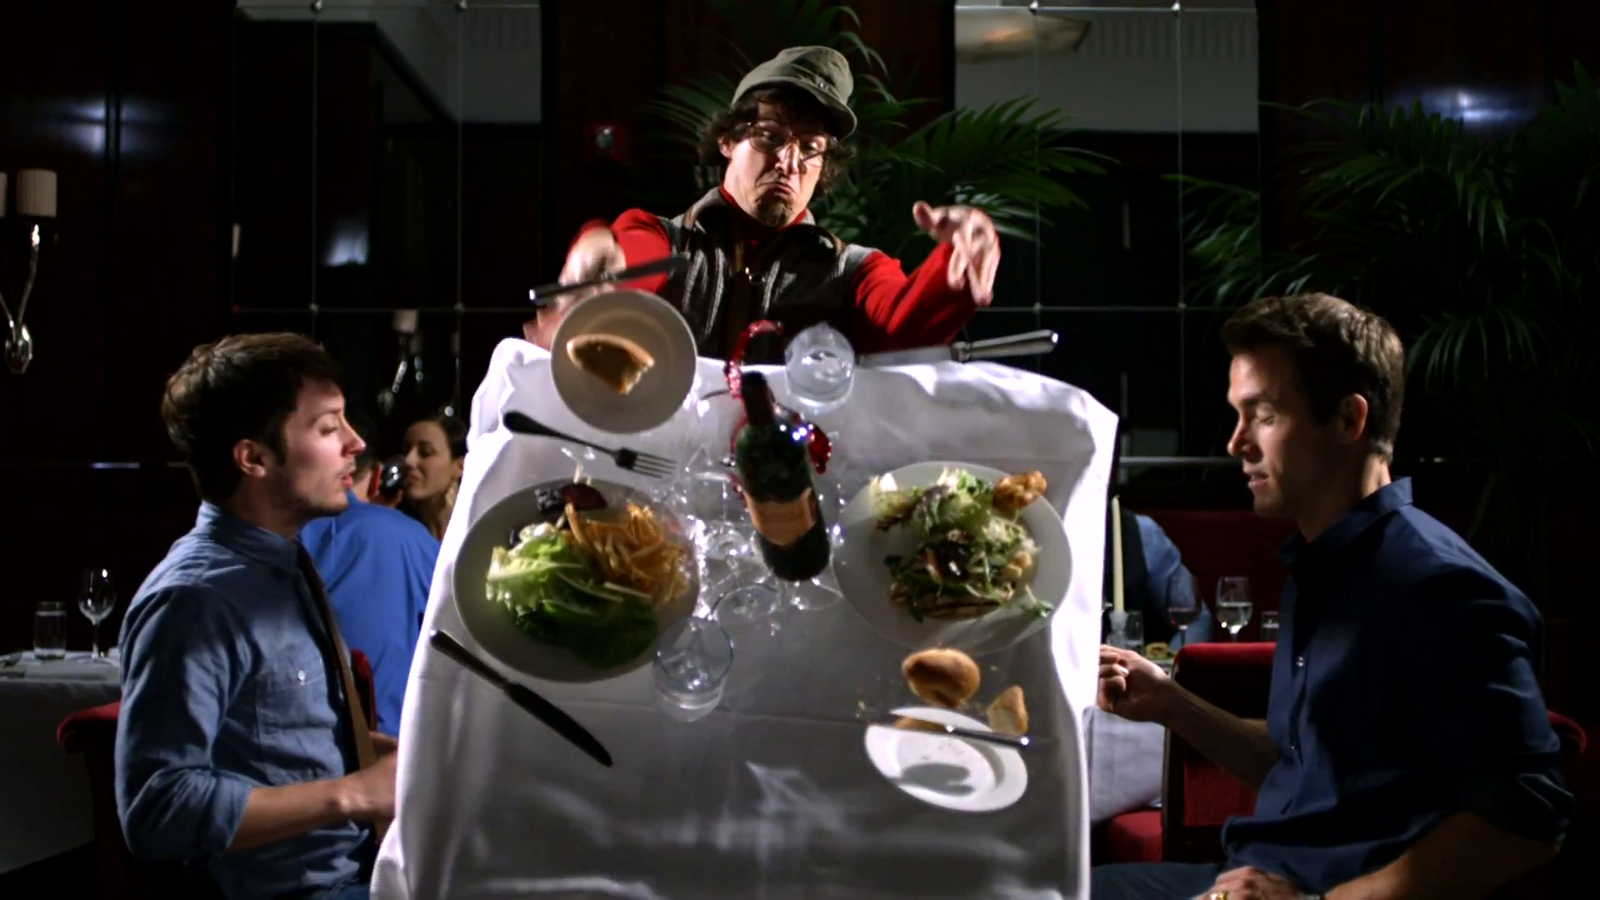
\includegraphics[width=\textwidth]{ground}
        \end{column}
    \end{columns}
\end{frame}

\begin{frame}{Attention mechanism}
    \begin{center}
        \begin{tikzpicture}[node distance=7mm, auto]
    % Encoder.
    \draw [cell, fill=orange!20] (-0.6, -0.8) rectangle (6.3, 0.45);

    % States.
    \node (e state1) [state] {$\s_1$};

    \foreach \i in {2, 3} {
        \pgfmathtruncatemacro{\j}{\i - 1}
        \node (e state\i) [state, right=of e state\j] {$\s_\i$};
    }

    \node (e state4) [block, right=of e state3] {$\cdots$};
    \node (e state5) [state, right=of e state4] {$\s_\tau$};

    \node [font=\small, left=of e state1] {encoder};

    % Inputs.
    \foreach \i in {1, ..., 3} {
        \node (e input\i) [state, below=of e state\i] {$\x_\i$};
    }

    \node (e input4) [block, below=of e state4] {$\cdots$};
    \node (e input5) [state, below=of e state5] {$\x_\tau$};

    \node (plus) [plus, above=of e state3] {};
    \node [left=2mm of plus, font=\small] {weighted average};

    % Decoder.
    \draw [cell, fill=orange!20] (-0.6, 1.9) rectangle (6.3, 3.15);

    \node (d state3) [state, above=of plus] {$\sh_{\th}$};
    \node (d state2) [state, left=of d state3] {$\sh_{\th-1}$};
    \node (d state1) [block, left=of d state2] {$\cdots$};
    \node (d state4) [state, right=of d state3] {$\sh_{\th+1}$};
    \node (d state5) [block, right=of d state4] {$\cdots$};

    \node [font=\small, left=of d state1] {decoder};

    % Arrows.
    \foreach\i in {1, ..., 5} {
        \draw [path] (e input\i) -- node [label, pos=0.7, right] {$\f$} (e state\i);
    }

    \draw [path] (e state1) -- node [label, above, pos=0.4] {$w_{\th 1}$} (plus);
    \draw [path] (e state2) -- node [label, right, pos=0.4, xshift=0.4mm] {$w_{\th 2}$} (plus);
    \draw [path] (e state3) -- node [label, right, pos=0.4, xshift=-1mm] {$w_{\th 3}$} (plus);
    \draw [path] (e state4) -- (plus);
    \draw [path] (e state5) -- node [label, above, pos=0.4] {$w_{\th \tau}$} (plus);

    \foreach\i in {2, ..., 5}{
        \pgfmathtruncatemacro{\j}{\i - 1}

        \draw [path] (e state\j) -- (e state\i);
        \draw [path] (d state\j) -- (d state\i);
    }

    \draw [path] (plus) -- node [right, pos=0.25] {$\c_{\th}$} (d state3);
\end{tikzpicture}
%%% Local Variables:
%%% mode: latex
%%% TeX-master: "../rnn"
%%% End:

    \end{center}

    \begin{itemize}
        \item At each $\th$ in the decoder, weighted average of $\s_1, \dots, \s_\tau$ forms context vector $\c_{\th}$
        \item Weights computed from trained alignment model
        \begin{itemize}
            \item Yields how well $\s_t$ \alert{aligns} with $\sh_{\th}$
        \end{itemize}
    \end{itemize}
\end{frame}

\begin{frame}{Embeddings}
    \begin{itemize}
        \item When classifying by one-hot encoding, all $c$ classes have identical $L^p$ distance from all others
        \item One-hot is fine for small $c$, but for large $c$, dim-$\tilde{c} \ll c$ \textcolor{Green4}{embeddings} generally do better
        \item E.g., \texttt{sheep} should have smaller distance to \texttt{ewe} or \texttt{goat} than to \texttt{quasar} or \texttt{supersonic}
        \item \textcolor{Green4}{Embeddings} can be pre-trained, or simultaneously trained with RNN
        \item Note: not at all unique to RNNs
    \end{itemize}

    \centering
    \begin{tikzpicture}[node distance=4.9mm, auto]
    % Embeddings.
    \node (e rnn 0) [lstm] {\rnn};

    \foreach \i in {0, ..., 4} {
        \pgfmathtruncatemacro{\j}{\i + 1}
        \node (e rnn \j) [lstm, right=of e rnn \i] {\rnn};
    }

    \foreach \i in {0, ..., 5} {
        \node (embed \i) [dense, below=of e rnn \i] {embed};
        \node (e output \i) [coordinate, above=of e rnn \i] {};
    }

    \node (e input 0) [word, below=of embed 0] {I};
    \node (e input 1) [word, below=of embed 1] {threw};
    \node (e input 2) [word, below=of embed 2] {it};
    \node (e input 3) [word, below=of embed 3] {on};
    \node (e input 4) [word, below=of embed 4] {the};
    \node (e input 5) [word, below=of embed 5] {ground};

    \node (e output) [coordinate, above=of e rnn 5] {};

    \foreach \i in {0, ..., 5} {
        \draw [path] (e input \i) -- node [label, right] {$\Reals^c$} (embed \i);
        \draw [path] (embed \i) -- node [label, right] {$\Reals^{\tilde{c}}$} (e rnn \i);
    }

    \foreach \i in {0, ..., 4} {
        \pgfmathtruncatemacro{\j}{\i + 1}
        \draw [path] (e rnn \i) -- (e rnn \j);
    }

    \draw [path] (e rnn 5) -- (e output);

    % Projections.
    \node (f rnn 0) [lstm, right=of embed 5] {\rnn};

    \foreach \i in {0, ..., 3} {
        \pgfmathtruncatemacro{\j}{\i + 1}
        \node (f rnn \j) [lstm, right=of f rnn \i] {\rnn};
    }

    \foreach \i in {0, ..., 4} {
        \node (f input \i) [coordinate, below=of f rnn \i] {};
        \node (project \i) [word, dense, above=of f rnn \i] {map};
    }

    \node (f output 0) [word, above=of project 0] {Je};
    \node (f output 1) [word, above=of project 1] {l'ai};
    \node (f output 2) [word, above=of project 2] {jet\'e};
    \node (f output 3) [word, above=of project 3] {par};
    \node (f output 4) [word, above=of project 4] {terre};

    \foreach \i in {0, ..., 4} {
        \draw [path] (f input \i) -- (f rnn \i);
        \draw [path] (f rnn \i) -- node [label, right] {$\Reals^{\tilde{d}}$} (project \i);
        \draw [path] (project \i) -- node [label, right] {$\Reals^d$} (f output \i);
    }

    \foreach \i in {0, ..., 3} {
        \pgfmathtruncatemacro{\j}{\i + 1}
        \draw [path] (f rnn \i) -- (f rnn \j);
    }
\end{tikzpicture}

%%% Local Variables:
%%% mode: latex
%%% TeX-master: "../rnn"
%%% End:

\end{frame}

%%% Local Variables:
%%% mode: latex
%%% TeX-master: "../rnn"
%%% End:
